\documentclass[12pt,
article,
type=sta, %sta, diplom, bsc, pp, msc, dr, drfinal, sem, prosem, bsc
colorbacktitle,
instlogo,
english,
accentcolor=tud9c,
%twoside
]{tudthesis}

\usepackage[english,ngerman]{babel}

\usepackage[T1]{fontenc}
\usepackage[utf8]{inputenc}

\usepackage[ngerman]{todonotes}
\usepackage{morefloats}
\usepackage{subcaption}

% linebreak for urls in bitex
\usepackage{url}
\urlstyle{rm}

%listings

\usepackage{listings}
\usepackage{xcolor}
\usepackage{babel,blindtext}
\usepackage{color}
\definecolor{lightgray}{rgb}{.9,.9,.9}
\definecolor{darkgray}{rgb}{.4,.4,.4}
\definecolor{purple}{rgb}{0.65, 0.12, 0.82}
\lstdefinelanguage{JavaScript}{
	keywords={break, case, catch, continue, debugger, default, delete, do, else, false, finally, for, function, if, in, instanceof, new, null, return, switch, this, throw, true, try, typeof, var, void, while, with},
	morecomment=[l]{//},
	morecomment=[s]{/*}{*/},
	morestring=[b]',
	morestring=[b]",
	ndkeywords={class, export, boolean, throw, implements, import, this},
	keywordstyle=\color{blue}\bfseries,
	ndkeywordstyle=\color{darkgray}\bfseries,
	identifierstyle=\color{black},
	commentstyle=\color{purple}\ttfamily,
	stringstyle=\color{red}\ttfamily,
	sensitive=true
}

\lstset{
	language=JavaScript,
	backgroundcolor=\color{lightgray},
	extendedchars=true,
	basicstyle=\footnotesize\ttfamily,
	showstringspaces=false,
	showspaces=false,
	numbers=left,
	numberstyle=\footnotesize,
	numbersep=9pt,
	tabsize=2,
	breaklines=true,
	showtabs=false,
	captionpos=b
}

\definecolor{pblue}{rgb}{0.13,0.13,1}
\definecolor{pgreen}{rgb}{0,0.5,0}
\definecolor{pred}{rgb}{0.9,0,0}
\definecolor{pgrey}{rgb}{0.46,0.45,0.48}

\lstset{language=Java,
	showspaces=false,
	showtabs=false,
	breaklines=true,
	showstringspaces=false,
	breakatwhitespace=true,
	commentstyle=\color{pgreen},
	keywordstyle=\color{pblue},
	stringstyle=\color{pred},
	basicstyle=\ttfamily,
	moredelim=[il][\textcolor{pgrey}]{\$\$},
	moredelim=[is][\textcolor{pgrey}]{\%\%}{\%\%}
}

\newcommand\JSONnumbervaluestyle{\color{blue}}
\newcommand\JSONstringvaluestyle{\color{red}}

% switch used as state variable
\newif\ifcolonfoundonthisline

\makeatletter

\lstdefinestyle{json}
{
	showstringspaces    = false,
	keywords            = {false,true},
	alsoletter          = 0123456789.,
	morestring          = [s]{"}{"},
	stringstyle         = \ifcolonfoundonthisline\JSONstringvaluestyle\fi,
	MoreSelectCharTable =%
	\lst@DefSaveDef{`:}\colon@json{\processColon@json},
	basicstyle          = \ttfamily,
	keywordstyle        = \ttfamily\bfseries,
}

% flip the switch if a colon is found in Pmode
\newcommand\processColon@json{%
	\colon@json%
	\ifnum\lst@mode=\lst@Pmode%
	\global\colonfoundonthislinetrue%
	\fi
}

\lst@AddToHook{Output}{%
	\ifcolonfoundonthisline%
	\ifnum\lst@mode=\lst@Pmode%
	\def\lst@thestyle{\JSONnumbervaluestyle}%
	\fi
	\fi
	%override by keyword style if a keyword is detected!
	\lsthk@DetectKeywords% 
}

% reset the switch at the end of line
\lst@AddToHook{EOL}%
{\global\colonfoundonthislinefalse}

\makeatother

\newcommand{\getmydate}{%
	\iflanguage{ngerman}{%
		\ifcase\month%
		\or Januar\or Februar\or M\"arz%
		\or April\or Mai\or Juni\or Juli%
		\or August\or September\or Oktober%
		\or November\or Dezember%
		\fi\ \number\year%
	}%
	\iflanguage{english}{%
		\ifcase\month%
		\or January\or February\or March%
		\or April\or May\or June\or July%
		\or August\or September\or October%
		\or November\or December%
		\fi\ \number\year%
	}
}
% changed counter for section wise counting
\usepackage{chngcntr}
\counterwithin{figure}{section} 
\counterwithin{table}{section} 

\setinstitutionlogo[height]{logo/tk_logo.jpg}

\usepackage{float}

\setlength{\parindent}{0pt} 

\begin{document}
	
	\renewcommand{\floatpagefraction}{.8}
	
	\selectlanguage{english}
	\counterwithin{lstlisting}{section}
	\thesistitle{Internet Praktikum - HOTEL Square}{Technical Documentation}
	
	\author{Tim Burkert, Christian Hack, Marco Huber, Truong, Robert Königstein}
	
	\referee{Prof. Dr. M\"uhlh\"auser}{Dipl.-Inform. Sebastian Kauschke}[M.Sc. Christian Meurisch]
	
	\department{\mbox{Department of Computer Science}\\ (FB20)\\\\\\\\Prof. Dr. M\"uhlh\"auser\\\ Hochschulstr. 10
		\\ 64289 Darmstadt \\\\www.tk.informatik.tu-darmstadt.de}
	\group{Telecooperation Group}
	
	\selectlanguage{ngerman}
	\makethesistitle
	\selectlanguage{english}
	\affidavit{Tim Burkert, Christian Hack, Marco Huber, Truong, Robert K\"onigstein}
	
	\cleardoublepage
	\listoftodos
	\cleardoublepage
	
	\pagenumbering{Roman}

	\cleardoublepage
	\tableofcontents
	\cleardoublepage
	\listoffigures
	\cleardoublepage
	\listoftables
	\cleardoublepage
	
	\pagenumbering{arabic}
	
	%all chapters	
	\section{Introduction}
\label{sec:introduction}
The following technical documentation will give further information for the implementation of the \textit{Internet Praktikum} from the group \texttt{HOTEL-Square}. The \textit{Internet Praktikum} aims at getting in touch with current web technologies, which "are becoming the basic building blocks of the next generation of Internet services"\footnote{\url{https://www.tk.informatik.tu-darmstadt.de/de/teaching/sommersemester-2017/internet-praktikum-tk-p4/}, 03.07.2017}. Therefore, state-of-the-art protocols and technologies are used to implement a specific task in a web based context.

\subsection{Task}
\label{subsec:task}
The task of the \textit{Internet Praktikum} in summer term 2017 is to reimplement a clone of the \textit{Foursquare Android} app. The task includes a well defined extend of compulsory features, which the app should support. There is the possibility of extending this compulsory feature list by some bonus features. 

In general, the task of the project includes the implementation of a well defined architecture, which comprises a development task for an \textit{Android} app (frontend) and a development task including a server in \textit{NodeJS} (backend). The backend should include a \textit{NoSQL} database and is allowed to query some third-party API-services. In opposite, the frontend is limited to communicate with the \textit{NodeJS}-server via some well-defined API. 
\newline\newline
The compulsory features of the app are:
\begin{itemize}
	\item User management:
	\begin{itemize}
		\item Create new account
		\item Login
		\item Delete account
		\item Reset password
	\end{itemize}
	\item Venue data:
	\begin{itemize}
		\item Pull venue data from the backend
	\end{itemize}
	\item Possible User Actions:
	\begin{itemize}
		\item Venue Search (at current location and in other location)
		\item Venue Search via text input and via predefined categories
		\item Search results must be displayed in a list and on a map
	\end{itemize}
	\item Venue view 
	\begin{itemize}
		\item Venue overview page showing photos and important information about the venue
		\item Look at photos that where uploaded to the venue in a photo albu with swiping
		\item Add comments with text and photos, like/dislike them and read other's comments
		\item Check into venues to show you where there
		\item Rate the venues
		\item Show the current top visitors of a venue
	\end{itemize}	
	\item Map
	\begin{itemize}
		\item Show venues on the map, click on them to get to the venue overview
		\item Show the user's location on the map
		\item Show the user's friends location on the map
	\end{itemize}
	\item User profile
	\begin{itemize}
		\item Profile view
		\item Profile fields containing the user name, real name, age and city
		\item Picture
		\item Profile editing for the user's own profile
	\end{itemize}
	\item Friends
	\begin{itemize}
		\item Find friends by name/user name, through comments on venues or on the map
		\item Friend list showing the user's friends with links to their profile
		\item Chat/messaging with the user's friends
	\end{itemize}
	\item Venue Gamification
	\begin{itemize}
		\item User with the must "checkins" in a venue is the "king"
	\end{itemize}
\end{itemize}

Proposed bonus features for the app are:
\begin{itemize}
	\item User management:
	\begin{itemize}
		\item Facebook/other login
		\item E-Mail confirmation
	\end{itemize}
	\item Search Results:
	\begin{itemize}
		\item must be filterable
	\end{itemize}
	\item Map
	\begin{itemize}
		\item Live update of the user's friends location
	\end{itemize}
	\item Friends
	\begin{itemize}
		\item Privacy measures
	\end{itemize}
	\item Venue Gamification
	\begin{itemize}
		\item Any gamification is a bonus
	\end{itemize}
\end{itemize}

The compulsory features of the server are:
\begin{itemize}
	\item Implementation of the server in \textit{NodeJS}
	\item Usage of a \textit{NoSQL} database for storage
	\item Implementation of a \texttt{REST}-ful API for the app-calls (\texttt{CRUD} for comments, ratings, pictures and ALL possible acitons)
	\item Hosting of the server
	\item Pull venue data from \textit{Google} (or similar service)	
\end{itemize}

\todo[inline]{finish introduction maybe with some general infos about Android, NodeJS, etc.}
	\cleardoublepage
	\section{Frontend}
\label{sec:frontend}

\subsection{Venues Search}
Venue Search is one of the main part of the application. When users want to search for their interest, they will experience two steps. The first is fast search and the second is deep search
Each step is taken by a Fragment \footnote{\url{https://developer.android.com/guide/components/fragments.html}}. Two fragments are working in the MainActivity and taking the different responsibilities for searching. In DeepSearchFragment is VenueStatePageAdapter which extends class FragmentStatePagerAdapter  \footnote{\url{https://developer.android.com/reference/android/support/v4/app/FragmentStatePagerAdapter.html}} provided  to manage switching two view modes, that are also two Fragments and are created or destroyed if necessary.
\begin{figure}[htbp]
	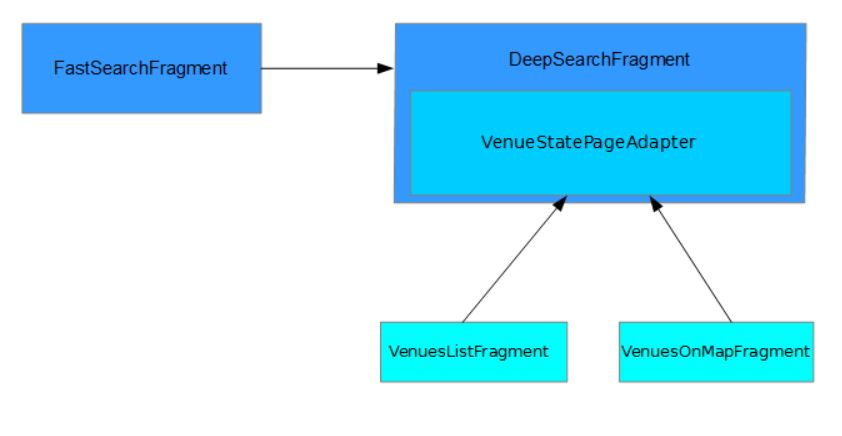
\includegraphics[width=0.8\textwidth]{images/venue_search.jpg}
	\centering
	\caption[]{Venue Search architecture}
	\label{fig:venue_search}
\end{figure}
\subsubsection{Fast Search}
When user starts the application, the fast search will be firstly displayed. It plays a role as default view of the application. It provides some name suggestions of interest which are written from static strings resource. On it five categories are predefined and each category contains three items (Figure \ref{fig:fastsearch}).
\begin{itemize}
	 \item Food and Drinks: beer, cafe, veggie
	 \item Holiday and Relaxation: beach, castle, zoo
	 \item Services: bank, gas station, car wash
	 \item Shops: supermarket, florist, music
	 \item Infrastructure: airport, harbor, e-charging station
\end{itemize}

 By clicking on one of the suggested name or search bar it will be redirected to Deep Search.
\begin{figure}[htbp]
	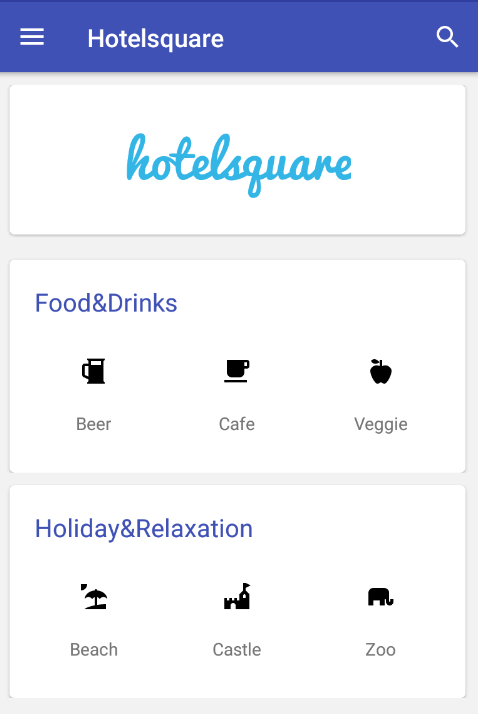
\includegraphics[width=0.8\textwidth]{images/fastsearch.png}
	\centering
	\caption[]{Fast Search with suggestion names of interest}
	\label{fig:fastsearch}
\end{figure} 
\subsubsection{Deep Search}

In order to find out venues, a query should be defined. It includes three parts, the first is keyword which can be name of interest selected in fast search or typed text in search bar in deep search, the second are filters, the last one is a page number. There are two types of filters, the location is mandatory and  radius, price and open now  are optional. The location can be the name of cities, countries or the current GPS value of users.
When user types text in search bar, the application will suggest some names of interest that are 
read from local database. When the app starts for the first time, the keyword suggestions  are read from static strings resource then inserted into local database\footnote{\url{https://developer.android.com/reference/android/database/sqlite/SQLiteDatabase.html}} with the help of green Dao \footnote{\url{http://greenrobot.org/greendao/}}. Additionally, they are also dynamically extracted from types of venues and typed text by the user which has been not located in the local database (Figure \ref{fig:keywordSuggestions}).

If the user doesn't have any input in location filter, the "near me" mode will be enabled. That means searching for all venues around the current location of the user by GPS value. It also plays a role as default search mode when redirecting from fast search to deep search. Otherwise, users have to give desired location name. However, it is not needed to give the complete meaningful location name, because this filter is surrounded by AutoCompleteTextView \footnote{\url{https://developer.android.com/reference/android/widget/AutoCompleteTextView.html}}. The application will take a suggested list of locations from the server then shows completion suggestions for the user (Figure \ref{fig:locationSuggestions}).
The page number is the pivot for obtaining corresponding number of venues. It is paremeterized in venue serivce. It will be clarifyed in the next section.
Deep search only processes in the following cases:
\begin{enumerate}
	\item Submit keyword in search bar
	\item Select keyword from suggested names
	\item Select item from suggested locations
	\item Change radius values
	\item Select and deselect price values(from 1 to 5)
	\item Select and deselect open now filter
\end{enumerate}


\begin{figure}[htbp]
	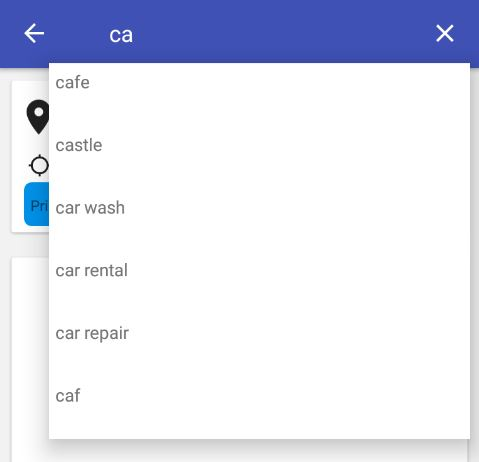
\includegraphics[width=0.8\textwidth]{images/suggestedkeywords.jpg}
	\centering
	\caption[]{Keyword suggestions}
	\label{fig:keywordSuggestions}
\end{figure} 

\begin{figure}[htbp]
	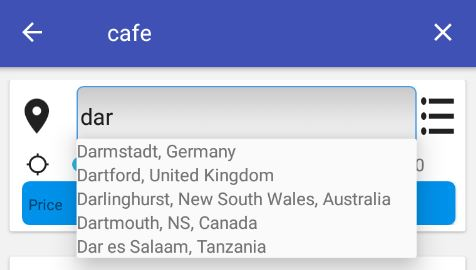
\includegraphics[width=0.8\textwidth]{images/suggestedlocations.jpg}
	\centering
	\caption[]{Location suggestions}
	\label{fig:locationSuggestions}
\end{figure} 
In order to avoid sending undesired request to the server, the current keyword will be saved as last keyword query. In cases 1 und 2, if the current keyword and the saved keyword query are the same, the request will be not sent. 

Two possible view modes are supported:
 \begin{enumerate}
 	\item Venues in list: For each request are only 10 venues returned. The first request starts with the page number 0 to obtain the first 10 venues. As the user scrolls list until an index position which modulo 10 is equals to 9, the page number will be increased by one and the next quest with the same content query will be sent. In this case are only the basic information( venue name, rating and venue image) displayed (Figure \ref{fig:venuesInlist}). If the user clicks on venue item, it will be redirected to venue in detail view.
 	\begin{figure}[htbp]
 		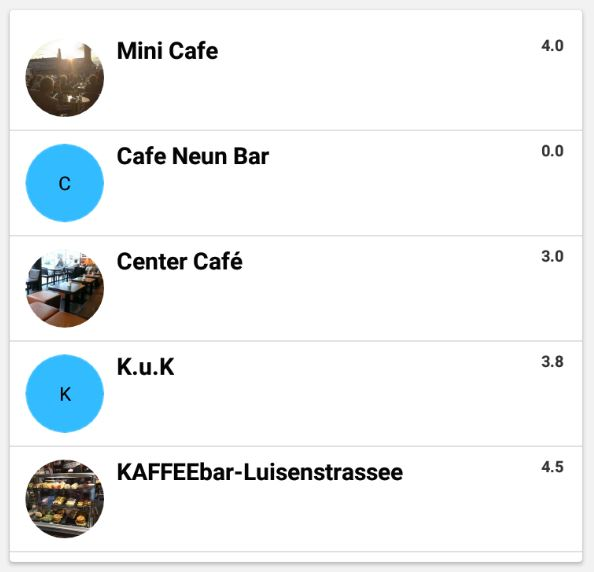
\includegraphics[width=0.8\textwidth]{images/venuesonlist.jpg}
 		\centering
 		\caption[]{Venues in list}
 		\label{fig:venuesInlist}
 	\end{figure}
 	\item Venues on map: it will be described in (\ref{markervenue})
 \end{enumerate}
There is a correlation between venues on map and venues in the list because only the first mode has an effect on changing the number of returned venues. If the user wants to see all venues pointed in the second mode, firstly he should enable or switch to the first mode then scroll to reach the maximal possible number of venues.

\subsection{Location Awareness}

To provide the possibility to find nearby venues and friends the application needs to be aware of the location of the user and his friends. A background service which tracks the location of the users has been implemented to achieve this. The location data is then provided to the search, the map and the server.

\subsubsection{LocationService}
The \textit{LocationService} is a simple background service which is started at the start of the app and is stopped when the \textit{MainActivity} is destoryed. The main functionality is to controll the \textit{LocationTracker} which actually tracks the location.

\subsubsection{LocationTracker}
The \textit{LocationTracker} is implemented as a \textit{LocationListener}. The \textit{GooglePlayService API} is used to obtain the location every interval. The interval is parameterized.

There are two different modes to guarantee a balance between power usage and accuracy. If the user is going to send a search request by starting to search for a venue, the priority of the \textit{GoogleAPI} client is set on high accuracy, otherwise and after the search, the mode is set on balance between accuracy and power usage. Moreover there is a check if the necessary permissions are provided or not. On every change of the location, the location is send as a \textit{LocationEvent} over the \textit{EventBus}. 

\subsection{Communication via greenrobot.org/EventBus}

To communicate between the service and the acticity and fragements the \textit{greenrobot.org/EventBus} is used. There are two different events which are posted on the bus and three different cases:


\begin{figure}[htbp]
	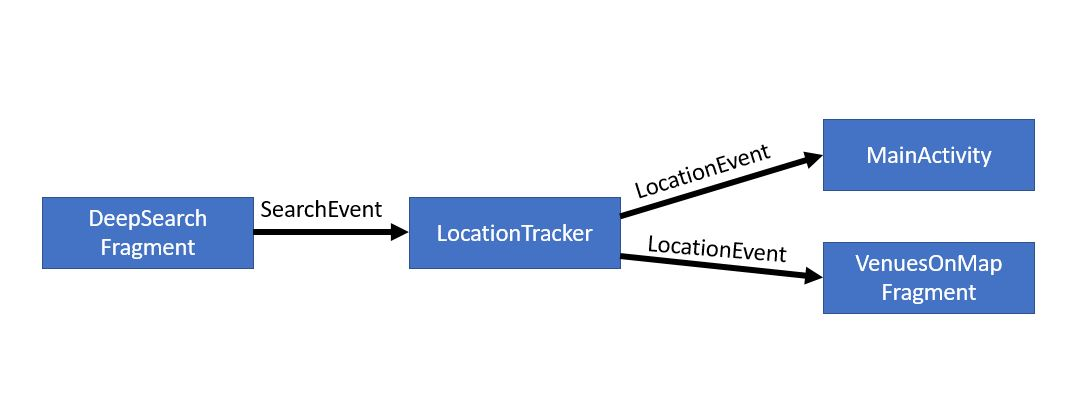
\includegraphics[width=0.8\textwidth]{images/eventBus.jpg}
	\centering
	\caption[]{\textit{EventBus} graph, schematically shows who sends which event type and who receives it}
	\label{fig:eventbus}
\end{figure} 


\begin{itemize}
\item The \textit{LocationTracker} subscribes on it to receive the \textit{SearchEvent}, which tells it to change the accuracy
\item The \textit{SearchEvent} is posted by the \textit{DeepSearchFragement} everytime its view is created
\item The \textit{LocationTracker} posts a \textit{LocationEvent} on the \textit{EventBus}, which contains the Location and is received by the \textit{MainActivity} and the \textit{VenueOnMapFragment}
\item The \textit{MainActivity} receives the \textit{LocationEvent}, stores it locally and sends it every 10 seconds (parameterized) to the server, to update the users position data
\item The \textit{VenueOnMapFragment} receives the \textit{LocationEvent} to update the location of the user on the map and also the location of his friends if the user is logged in
\end{itemize}

\subsection{The Map} \label{markervenue}
The map is used as a function to show the user graphically where he and his nearby friends are and also the searched venues. The functionality of the map in inside the \textit{VenuesOnMapFragment}, which is part of the \textit{MainActivity}. The map itself is provided by \textit{GoogleMaps}.

There are three different kinds of markers shown on the map. If the user clicks on any marker, a button shows up, which allows him to change to \textit{GoogleMaps} and gets the route to the chosen marker. 

\subsubsection{Marker: Venue} 
The venue markers locate the search results on the map. They differ in color, depending on the rating of the venue. Those colors are with the following more or less obvious order:

\begin{itemize}
\item \textbf{grey}: No rating available / no rating yet
\item \textbf{red}: rating between 0 and 1
\item \textbf{orange}: rating between 1 and 2
\item \textbf{yellow}: rating between 2 and 3
\item \textbf{lime}: rating between 3 and 4
\item \textbf{green}: rating between 4 and 5
\end{itemize}

If the user clicks on one of the markers an infoWindow shows up, which shows on image and tells the name, the exact rating and if it is open right now or not. With a click on the infoWindow the user is redirected to the \textit{VenueDetails}, where he can find more additional information about the venue.

\subsubsection{Marker: Friend}
The friend markers locate the friends of the user, if he is logged in and has nearby friends. The marker of the friends is similar to the marker of the user, except it is green.
The position of his nearby friends are updated everytime, the location of the user changes. 

If the user clicks on on of his friends marker, an \textit{infoWindow} shows up with the avatar and name and if given, also the city and age. With a click on the \textit{infoWindow} the user gets to the profile of his friend.

\subsubsection{Marker: User}
The user marker locate the user on the map. If the user clicks on himself, a \textit{infoWindow} shows up. If the user is not logged in, it shows the default \textit{infoWindow} with the default avatar. If the user is logged in, it shows his own avatar and additonal info. 

If he clicks on the \textit{infoWindow} he is redirected to his own profile.

\begin{figure}[htbp]
 	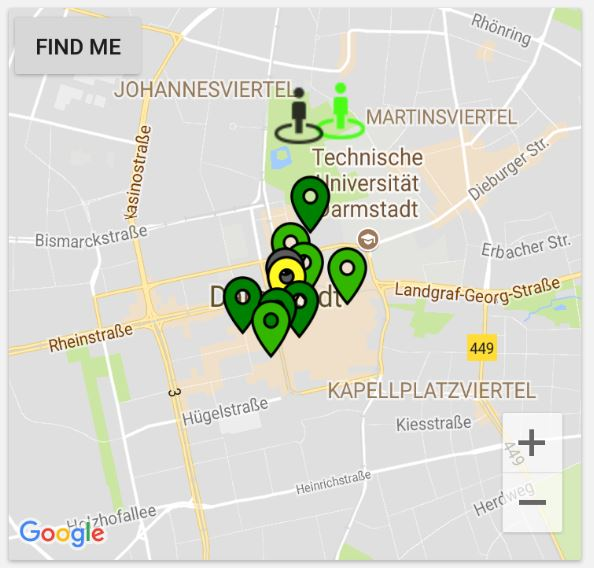
\includegraphics[width=0.8\textwidth]{images/venuesonmap.jpg}
 	\centering
 	\caption[]{Venues, friends and user on map}
 	\label{fig:venuesonmap}
\end{figure}



\subsection{Venue in detail}
By detailing informations of venue, the use not only getting more meaningful information but can also do more actions on it. The informations are distributed in two parts. The first one is the detailed about venue; including name, address, number of check-ins, price level and images.
In addition to it, the location is also pointed on a small map. By clicking on location on map the user can always directly utilize two optional functionalities of Googlemap. With the same action on Call Button he can also make a phone call to owner of venue or check in, if he is interested in it (Figure \ref{fig:detailedInformationsOfVenue}).
\begin{figure}[htbp]
	\includegraphics[width=0.8\textwidth]{images/venueInDetail_Part_1.jpg}
	\centering
	\caption[]{Detailed informations of venue}
	\label{fig:detailedInformationsOfVenue}
\end{figure}

The second part is the previous activities of users on venue. That consits of a leaderboard of three available check-ins, top-ten check-ins and list of comments( text comments and image comments). The leaderboard is sorted by the number of users check-ins. The two others are sorted by decreasing order of time. On each comment two like and unlike buttons are provided, therefore the user can consider to do actions on it. From this view, if he clicks on profile or username, he will be redirected to the selected user profile(Figure \ref{fig:previous_activities}).
The last one is floating menu user activities. With floating menu\footnote{\url{https://github.com/Clans/FloatingActionButton}} it is possible to minimize the spaces on the view and floating buttons will appear when these are needed according to opinion of the user. Moreover, in any time he can post text(Figure \ref{fig:textcomment}) or image(Figure \ref{fig:imagecomment}) on this venue or can obtain all images of venue(Figure \ref{fig:overimages}). On the overview of images the user can see fullscreen image by swiping left or right on selected image(Figure \ref{fig:swipeimage}).

\begin{figure}[htbp]
	\includegraphics[width=0.8\textwidth]{images/venueInDetail_Part_2.jpg}
	\centering
	\caption[]{The previous activities of users on venue}
	\label{fig:previous_activities}
\end{figure}

\begin{figure}[!htb]
	\minipage{0.45\textwidth}
	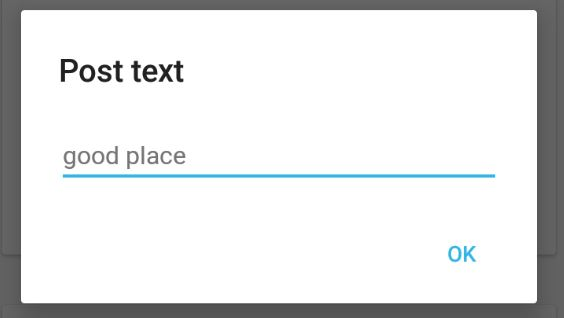
\includegraphics[width=\linewidth]{images/textcomment.jpg}
	\caption{Text comment}\label{fig:textcomment}
	
\includegraphics[width=\linewidth]{images/imagecomment.jpg}
	\caption{Image comment}\label{fig:imagecomment}
	\endminipage\hfill
	\minipage{0.45\textwidth}
	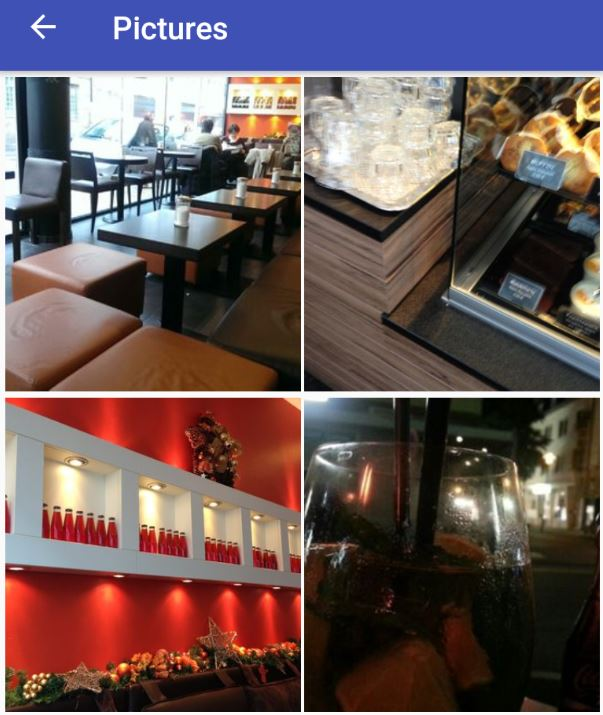
\includegraphics[width=\linewidth]{images/overview_image.jpg}
    \caption{Overview pictures}\label{fig:overimages}
	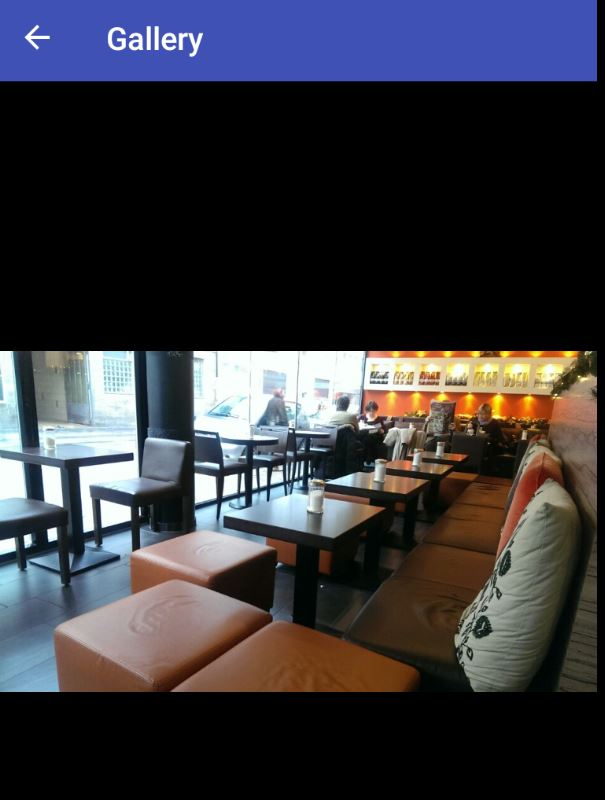
\includegraphics[width=\linewidth]{images/swipeimage.jpg}
	\caption{Swiped picture}\label{fig:swipeimage}
	\endminipage\hfill

\end{figure}

\subsection{History}
History section is built with the purpose to help users tracking their activities on venues. In the implementation  only activities of logged-in users are saved in local database. Assuming that a smart device can be identified with a being logged-in user. This means that only state of user is taken into account. In order to distinguish the activities on venue, the five following states are defined:

\begin{itemize}
	\item CHECK IN(0)
	\item LIKE COMMENT(1)
	\item DISLIKE COMMENT(2)
	\item TEXT COMMENT(3)
	\item IMAGE COMMENT(4)
\end{itemize}

Each history entry consits of five elements: history id, venue name, name  of activity, date of activity and referenced venue id. The green Dao takes responsibility for saving, deleting history entries. 
\begin{figure}[htbp]
	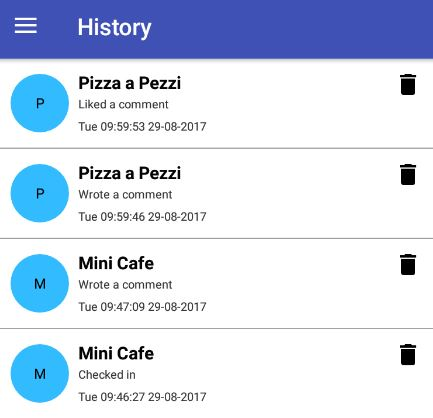
\includegraphics[width=0.8\textwidth]{images/history.jpg}
	\centering
	\caption[]{History activities}
	\label{fig:history}
\end{figure}
\subsection{Settings}
The SettingsFragment mainly provides three functionalities for logged-in users.

\begin{itemize}
\item \textbf{Language Selection:} The user has the ability to change the language of the app. There are two different languages supported: \textit{Deutsch} and \textit{English}. With a simple spinner he can change the app to his preferred language. Technically the language than is stored in the local storage and the strings are changed depending on that value.
\item \textbf{Incognito-Mode:} The \textit{Incognito-Mode} provides the user more privacy by not showing his position to anyone especially his nearby friends. The mode ist selected by a CheckBox to toggle the \textit{Incognito-Mode} The information, that the user wants to be not seen by anyone is then send to the server.
\item \textbf{Delete Profile:} This button provides the user the opportunity to delete his \textit{HOTELsquare} account. If he clicks on it, a dialog is open to make sure he knows what he is doing. If he confirm his choice, his profile is deleted, otherwise nothing happens.
\end{itemize}

The language selection is also available for user without a \textit{HOTELsquare} account.



	\cleardoublepage
	\section{Backend}
\label{sec:backend}
\todo[inline]{Backend technical documentation}
	\cleardoublepage
	
	
	%\bibliographystyle{alphadin}
	%\bibliography{literature}
	
	%\begin{appendix}
	%\section{Erster Anhang}
	%\end{appendix}
	
\end{document}
